\scanpage{43}
UNIVERSITE\\
DES SCIENCES ET TECHNIQUES\\
DU LANGUEDOC\\
\rule{2cm}{0.4pt}

Montpellier, le 15 Juin 1978

MR/FP

\uline{Diffusion}: Liste A\\
n$^{\circ}$ 3762

\uline{AVIS DE SOUTENANCE D'UNE THESE DE DOCTORAT}\\
\uline{D'UNIVERSITE}

\uline{Nom et Prénom du candidat} : GOUSSOPOULOS Jean

\uline{Titre de la thèse} : Etude de la croissance relative postnatale chez le poulet.\\
Principaux tissus et organes, muscles et os individuels. Influence de l'hypophy-\\
sectomie.

\uline{Date, heure et lieu de soutenance prévus} : 5 Juillet 1978 à 9 heures - U.S.T.L.\\
MONTPELLIER - ENSAM. Laboratoire Zootechnie.

\uline{Nom du Directeur de thèse} : L. DAUZIER

\uline{Désignation du laboratoire où la thèse est préparée} : Station de Physiologie Ani-\\
male - INRA - MONTPELLIER

\uline{Analyse de l'ouvrage} : Etude descriptive par l'utilisation d'allométrie, de la\\
croissance pondérale relative chez le poulet : principaux tissus et organes ;\\
os et muscles individuels. Mise en évidence de gradients de croissance et de dif-\\
férences de développement selon le sexe. Effets de l'hypophysectomie, dont l'in-\\
fluence est surtout nette au niveau du muscle et du tissus gras.

\uline{Durée approximative des recherches ayant abouti à la thèse} : 5 ans

\uline{Composition du jury proposé} :
\begin{tabular}[t]{l}
L. DAUZIER, Président\\
C. THIBAULT\\
J.D. BAYLE\\
M. BENEVENT
\end{tabular}

Le Secrétaire Général,
\figure{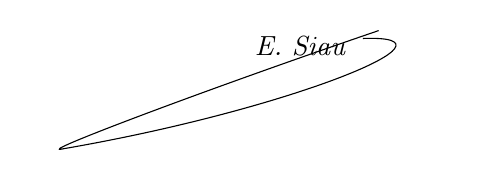
\begin{tikzpicture}[x=1cm,y=1cm]
\node[font=\itshape] at (3.1,.65) {\unsure{E. Siau}};
\draw (3.9,.75) .. controls (5.3,.8) and (3,-.15) .. (.1,-.65)
 .. controls (-.35,-.75) and (1.9,.1) .. (4.1,.85);
\end{tikzpicture}}
\uline{E. SIAU.}
% archive foliation: 42
